\documentclass[11pt]{aghdpl}
% \documentclass[language=en,11pt]{aghdpl}  % praca w języku angielskim


%---------------------------------------------------------------------------

\author{Piotr Seemann}
\shortauthor{P. Seemann}

%\titlePL{Przygotowanie bardzo długiej i pasjonującej pracy dyplomowej w~systemie~\LaTeX}
%\titleEN{Preparation of a very long and fascinating bachelor or master thesis in \LaTeX}

\titlePL{Automatyczne odkrywanie procesów biznesowych przy użyciu programowania genetycznego}
\titleEN{Automated Business Process Discovery using Genetic Programming}


\shorttitlePL{Automatyczne odkrywanie procesów biznesowych przy użyciu programowania genetycznego} % skrócona wersja tytułu jeśli jest bardzo długi
\shorttitleEN{Automated Business Process Discovery using Genetic Programming}

\thesistype{Projekt dyplomowy}
%\thesistype{Master of Science Thesis}

\supervisor{dr inż. Krzysztof Kluza}

\degreeprogramme{Informatyka}
%\degreeprogramme{Computer Science}

\date{2021}

\department{Katedra Informatyki Stosowanej}
%\department{Department of Applied Computer Science}

\faculty{Wydział Elektrotechniki, Automatyki,\protect\\[-1mm] Informatyki i Inżynierii Biomedycznej}
%\faculty{Faculty of Electrical Engineering, Automatics, Computer Science and Biomedical Engineering}

\setlength{\cftsecnumwidth}{10mm}

%---------------------------------------------------------------------------
\setcounter{secnumdepth}{4}
\brokenpenalty=10000\relax

\begin{document}

\titlepages

\RedefinePlainStyle

\setcounter{tocdepth}{2}
\tableofcontents
\clearpage


\chapter{Wprowadzenie}
\label{cha:wprowadzenie}

%---------------------------------------------------------------------------

\section{Zarys tematyki pracy}
\label{sec:zarysPracy}
procesach biznesowych, co to, po co, gdzie się ich używa


\section{Cele pracy}
\label{sec:celePracy}

Celem pracy jest projekt i implementacja metody odkrywania procesów biznesowych przy użyciu programowania genetycznego. W pracy zbadano jak wybór metod programowania genetycznego, wybór gramatyki, a także parametrów programu wpływa na jakość rozwiązania. Zaprezentowano też przykłady użycia algorytmu do okrywania procesów biznesowych oraz porównano z innymi dostępnymi algorytmami. Ponadto w pracy zostały zbadana hipoteza czy rozwiązywania problemu najpierw dla prostych przypadków i wykorzystanie rozwiązań tego problemu może mieć korzystny wpływ na rozwiązanie bardziej skomplikowanego problemu.
%---------------------------------------------------------------------------

\section{Zawartość pracy}
\label{sec:zawartoscPracy}

Praca zastała podzielona na cztery części. We wstępie teoretycznym zostały przybliżone zagadnienia potrzebne do zrozumienia pracy. W kolejnej części została przedstawiona implementacja algorytmu do wyszukiwania procesów genetycznych. Następnie zaprezentowane zostały wyniki działanie algorytmu dla przykładowych dzienników zdarzeń. Omówione zostało też jak na czas znajdowania rozwiązania oraz jego jakość wpływają przyjęte parametry algorytmu w szczególności wybór metryk oraz wagi z jakimi każda metryka powinna być brana pod uwagę.  



















\chapter{Wstęp teoretyczny}
\label{cha:wstepTeoretyczny}

%---------------------------------------------------------------------------

\section{Procesy biznesowe}
\label{sec:procesyBiznesowe}

\subsection{Procesy biznesowe}
W każdym dużym przedsiębiorstwie, każdego dnia, wykonywana jest ogromna ilość czynności koniecznych do funkcjonowania tej organizacji. Ludzie oraz oraz systemy podejmują najróżniejsze działania związane z różnymi, często nie mającymi wiele wspólnego zadaniami. Mogą to być działania jak obsługa płatności, obsługa zamówień, wytwarzanie produktów czy ich transport. Przykłady te można mnożyć w zależności od sektora w jakim obraca się dana firma. Im jest ona większa, tym trudniej jest osobom zarządzającym opisać czy zrozumieć poszczególne czynności. W pewnym momencie, kiedy ilość rożnych zadań rośnie do setek czy tysięcy staje się to niemożliwe i potrzebny jest sposób na zebranie wiedzy o pojedynczych operacjach i opisanie jej za pomocą uporządkowanej struktury. Stąd narodził się pomysł na wykorzystanie wykorzystanie procesów biznesowych.

Procesy biznesowe opisują zbiór aktywność, które podejmuje grupa podmiotów w celu osiągnięcia celu biznesowego. W literaturze brakuje jednej ogólnie przyjętej definicji procesu biznesowego. W latach 90. XX wieku proponenci BPR, czyli Przeprojektowania procesów biznesowych (\textit{eng. Business process re-engineering}) starali się sprecyzować pojęcie procesu biznesowego. W książce "Process Innovation: Reengineering Work through Information Technology"\cite{davenport1993process} Davenport określił termin ten jako "Ustrukturyzowany, mierzalny zbiór działań, których celem jest wytworzenie określonego produktu dla określonego klienta lub rynku". Autor położył nacisk na zbiór kroków prowadzących do celu, raczej niż na końcowy efekt. W dalszej części autor pisze "Proces jest zatem określonym uporządkowaniem czynności roboczych w czasie i przestrzeni, z początkiem i końcem oraz jasno określonymi wejściami i wyjściami: strukturą działania.". Inni pionierzy BPR Michael Hammer i James Champy proponują podejście „Proces biznesowy to zbiór działań, który pobiera jeden lub więcej rodzajów danych wejściowych i tworzy wynik, który ma wartość dla klienta”\cite{HAMMER199390}. Autorzy dają większą dowolność, co do definicji procesu, nie wspominając o konieczności jego logicznej organizacji czy mierzalności. Z kolei Jacobson zupełnie pomija konieczność zamknięcia procesu w jakiekolwiek ramy: "Zestaw czynności wewnętrznych wykonywanych w celu obsługi klienta"\cite{JacobsonObjectAdvantage}. Nacisk na konieczność odniesienia procesów do wymiernych środków firmy widzimy w definicji: "Procesy biznesowe są aktywną częścią biznesu. Opisują funkcje firmy i obejmują zasoby, które są używane, przekształcane lub wytwarzane. Proces biznesowy to abstrakcja, która pokazuje współpracę między zasobami i transformację zasobów w biznesie. Podkreśla, w jaki sposób wykonywana jest praca, zamiast opisywać produkty lub usługi wynikające z tego procesu."\cite{Eriksson2000BusinessMW}. Szczególnie ważny jest tutaj fragment o transformacji zasobów, gdyż każe on rozumieć poszczególne aktywności w procesie jako powiązane ze sobą i kończące się namacalnymi rezultatami. Definicja "Proces biznesowy to seria kroków mających na celu wytworzenie produktu lub usługi. W wyniku niektórych procesów produkt lub usługa jest odbierana przez zewnętrznego klienta organizacji. Nazywamy te podstawowe procesy. Inne procesy wytwarzają produkty, które są niewidoczne dla klienta zewnętrznego, ale są niezbędne do efektywnego zarządzania firmą. Nazywamy te procesy wsparcia"\cite{rummler_brache_1995} wprowadza rozgraniczenie na podtypy procesów. Ważnym jest jednak że nie jest koniecznością, aby rezultaty procesu były widoczne na zewnątrz organizacji.  

Powyższe definicji skupiają się na delikatnie odmienny aspektach procesów biznesowych, nie zawsze szczegółowo wspominając o innych. Starając się usystematyzować powyższe sformułowania, chcąc zbudować bazę do dalszej analizy tematu, można przyjąć, że procesy biznesowe charakteryzują:
\begin{itemize}
  \item[•] Określony cel, którym jest wytworzenie wartości dla klienta zewnętrznego lub pośrednio firmy - klienta wewnętrznego. Jednak warto jeszcze raz zaznaczyć ze proces biznesowy skupia się na sposobie osiągnięcia celu, a nie opisie celu samego w sobie. 
  \item[•] Dyskretny, jasno zdefiniowany i identyfikowalny zbiór aktywności. 
  \item[•] Jasno określony początek - wejście i koniec - wyjście.
  \item[•] Pomiędzy kolejnymi procesami zachodzi zależność przyczynowo-skutkowa.
\end{itemize}

Żeby lepiej zilustrować czym jest proces biznesowy, poniżej znajduje się prosty przykład często spotykanego procesu. Oczywiście, prawdziwy proces będzie posiadał o wiele więcej aktywności.

\begin{figure}[h]
	\centering{\includegraphics[scale=0.7]{simple-business-process.png}}
	\caption{\label{fig:subcaption_example}Przykład prostego procesu}
\end{figure}

Zauważmy, że mamy jasno zdefiniowany wejście - otrzymanie zamówienia od klienta oraz wyjście, kiedy dostarczamy oczekiwaną wartość dla klienta, a całość składa się z serii tworzących logiczną całość aktywności. Aktywności są konkretnie zdefiniowane. Standardem jest definiowanie aktywności w formie równoważników zdań.


\subsection{Zarządzanie procesami biznesowymi}
Zdefiniowanie proces biznesowego otwiera wiele możliwości analizy działań przedsiębiorstwa i w skutek tego wprowadzanie usprawnień. Dziedziną, która się tym zajmuje jest zarządzanie procesami biznesowymi (\textit{eng. Business process modeling}) zwane w skrócie BPM jest dziedziną. Sercem jest proces, a sam BPM może określić jako zbiór metod, technik i sposobów służący do projektowania, wprowadzania w życie, zarządzania i analizy procesów biznesowych\cite{BPMDemystified}. 

Celem stosowania metod zarządzanie procesami biznesowym jest 
Metoda te są obecnie szeroko stosowane przez organizacje i uznawane za arcyważną składową sukcesu danego podmiotu. 
Ważny jest człowiek
W publikacji \cite{SixElementsBPM} wyróżniono 6 podstawowych elementów BPM. Są to dopasowanie strategiczne, zarządzanie, modelowanie, techniki informatyczne, ludzie, kultura. Cześć z tych elemetów jest niezbyt ściśle zdefiniowiowane i wymaga bardziej ogólnego podejście, jednak do części z nich można z pomyślnością zastosować metody informatyczne. I dlatego to i to zaczęło czerpać ze zdobyczy informatyki
\cite{BPMWhat}
Business process lifecycle
W dalszej cześci pracy przedstawione zostaną sposoby na wykorzystanie d
%---------------------------------------------------------------------------

\section{Modelowanie procesów biznesowych}
\label{sec:modelowanie}
\subsection{Notacja}
Najpopularniejszą notacją używaną do opisu procesów biznesowych jest BPMN. 
W tutajbadanie opisano najpopularniejsze elementy używane w BPMN. 
\subsection{Modelowanie procesów biznesowych}
Przyjrzyjmy się sytuacji, w której klient chce naprawić pralkę. Klient initializuje proces naprawy kontaktując się z firmą naprawiającą sprzęt AGD. Rezulty tego procesu mogą być 2 : naprawiona i nie, a sam proces może się wykonać na duża ilość sposobów, to sprawia, że proces rośnie i potrzebne są metoda na uporządkowanie tego procesu w celu chociażby zwiększenia wydajności.

Grafika skomplikowanego procesu

Jest to szeroko pojęta dziadzina, która zawiera różne aplikacje metoda informatyki do procesów. 
Wyróżnia 3 podkategorie: odkrywanie, conformance checking 
Odkrywanie procesów
Metryki ważne

\subsection{Dzienniki zdarzeń}

\begin{figure}[h]
	\centering{\includegraphics[scale=0.8]{event-log.png}}
	\caption{\label{fig:subcaption_example}Przykład dziennika zdarzeń}
\end{figure}s

W kontekście odkrywania procesów biznesowych ważne są dla nas tylko zdarzenia i kolejność ich wykonywania. Informacje o dokładnym czasie wykonania oraz użytkowniku, który wykonał daną operację możemy pominąć. Ponadto musimy wiedzieć jak często dany wariant wystąpił.

\subsection{Odkrywanie procesów biznesowych}

Odkrywanie procesów biznesowy jest podgrupą i obejmuję techniki przekształcania danych w procesy.
Procesy zaprojektowane nie zawsze są realizowane w praktyce. Ważne jest, żeby proces był oparte tam analizie prawdziwych danych, a nie spekulacjach i założeniach.

\begin{figure}[h]
	\centering{\includegraphics[scale=0.5]{model-vs-real.png}}
	\caption{\label{fig:subcaption_example}Proces rzeczywisty i pierwotnie zakładany}
\end{figure}

\subsection{Algorytmy do wykrywania procesów biznesowych}
Alpha algorithm \newline
The ILP Miner \newline
Heuristic Miner \newline
Multi-phase Miner \newline


%---------------------------------------------------------------------------

\section{Metryki}
\label{sec:metryki}
\cite{doi:10.1142/S0218843014400012}
\subsection{Prostota}
Najprostsza z metryk. \newline
$M_{pro} = 1 - \frac{ilosc\ duplikatow\ w\ modelu\ +\ ilosc\ brakujacych\ wartosci\ w\ modelu}{ilosc\ unikalnych\ zdarzen\ w\ logu\ +\ ilosc\ zdarzen\ w\ modelu}$
\subsection{Odwzorowanie}
Pozostałe metryki obliczane są na podstawie tej metryki. \newline
$M_o = (1 - \sum_{0}^{ilosc\ procesow\ w\ logu} \frac{blad\ odwzorowania\ logu\ w\ modelu}{minimalna\ długosc\ sciezki\ w\ modelu\ +\ długosc\ sciezki\ w\ logu})^4$

Przykład liczenia odwzorowania: \newline

\subsection{Precyzja}

$M_{pre} = (1 - \sum_{0}^{ilosc\ zdarzen\ w\ modelu} \frac{ilosc\ osiagalnych\ zdarzen\ w\ modelu - ilosc\ osiagalnych\ zdarzen\ w\ logu}{ilosc\ osiagalnych\ zdarzen\ w\ modelu})^{\frac{1}{3}} $
\subsection{Generalizacja}
$M_g = \frac{1 - \sum_{0}^{ilosc\ zdarzen\ w\ logu} \frac{1}{\sqrt{ilosc\ wystapien\ zdarzenia}}}{ilosc\ zdarzen\ w\ logu} $
\subsection{Złożoność}
Promuje rozwiązywanie prostych problemów w prosty sposób \newline
$M_z = 1 - \frac{1}{\sqrt{1 - odwzorowanie\ *\ \sqrt{zlozonosc\ modelu}}} $


%---------------------------------------------------------------------------

\section{Ewolucja genetyczna}
\label{sec:ewolucjaGenetyczne}
\subsection{Algorytmy genetyczne}
\cite{ryan_collins_neill_1998}
Algorytmy genetyczne są inspirowaną selekcją naturalną  heurystyką, która używa znanych z ewolucji biologicznej operacji jak mutacja, selekcja czy krzyżowanie do rozwiązywania problemów wyszukiwania i optymizacji. Ich ideą jest zaproponowanie metody przeszukiwania przestrzeni losowy rozwiązań w celu wyszukania najlepszych z nich. Pierwszy raz zostały zaproponowane w \cite{10.5555/138936}.

Sposób działania algorytmów genetyczny polega na stworzeniu populacji losowych rozwiązań zwanych genotypami lub chromosomami, które kodowane są za pomocą licz całkowitych i zapisywane ww tablicy jednowymiarowej. Następnie dla każdego elementu populacji obliczane są metryki pozwalające ocenić jak dobre jest wygenerowane rozwiązanie. Po sklasyfikowaniu rozwiązań generujemy nową populację mutując lub krzyżując głownie choć nie tylko najlepsze chromosomy. Proces ten jest powtarzany do momentu otrzymania satysfakcjonującego rozwiązania.  

Selekcja:
Selekcja proporcjonalna - wybieramy losowo rozwiązania z puli wszystkich rozwiązań z warunkiem, że rozwiązania z największą wartością metryk mają największą szansę na bycie zachowanymi w populacji. Jest to najpopularniejsza metoda selekcji i najczęściej umożliwiająca najszybsze znalezienie rozwiązania. Pozwala na elityzm, czyli zachowanie części najlepszych genotypów w przyszłej populacji.

Selekcja turniejowa - wybieramy podzbiór ze zbioru rozwiązań i zachowujemy w przyszłej najlepsze rozwiązanie z tego podzbioru.
Rozwiązanie to pozwala na duży wpływ na presję genetyczną - zwiększając wielkość podzbioru ograniczamy szansę na wybór z niską wartością metryk.  Jest to także metoda, która łatwe zrównoleglenie.

Krzyżowanie - :
Krzyżowanie punktowe - spośród dwóch genotypów losowo wybieramy jeden punkt, następnie tworzymy dwa nowe genotypy pierwszy z chromosomów na prawo od punktu w pierwszym genotypie i na lewo w genotypie drugim oraz drugi z dwóch pozostałych.

Krzyżowanie dwupunktowe - spośród dwóch genotypów losowo wybieramy dwa punkty, następnie część pomiędzy tymi punktami jest zamieniana pomiędzy genotypami.

Krzyżowanie n-punktowe - uogólnienie powyższych krzyżowań dla n punktów.

Krzyżowanie zamiana w drzewie - genotyp może być reprezentowany jako drzewo, w tej metodzie zamieniamy ze sobą dwa poddrzewa, tworzone są tylko prawidłowe rozwiązania, jednak jest to metoda wymagająca większej ilości obliczeń. 


Mutacja:
Mutacja punkowa - dowolna wartość w tablicy zostaje zmieniona na inną losową wartość. Pozostałe produkcje pozostają niezmienione.

Mutacja zamiana w drzewie - genotyp może być reprezentowany jako drzewo, w tej metodzie tworzone jest nowe poddrzewo, przy tej metodzie tworzone są tylko prawidłowe rozwiązania, jednak jest to metoda wymagająca większej ilości obliczeń. 

 
  
\subsection{Ewolucja genetyczna a inne algorytmy uczenia maszynowego}
Algorytmy genetyczne pozwalają przeszukać najszerszą przestrzeń rozwiązań. Pozwalają na znajdowanie nieoczywistych rozwiązań.  
Inna heurystyką, która używa losowo rozwiązuje problem jest simulated annealing. Algorytm genetyczny jest łatwy w zrównogleniu i pozwala znaleźć globalne rozwiązanie.
Sieci neuronewe:
Pula rozwiązań zamiast jednego rozwiązywania. Szersze przeszukiwanie rozwiązań. 
\subsection{Ewolucja gramatyczna}
Ewoluuje gramatykę za pomocą metod ewolucji genetycznej w celu znalezienia programu, który najlepiej rozwiązuje problem.
Podejście to zostało zaproponowane w \cite{ryan_collins_neill_1998}. 

%---------------------------------------------------------------------------

\section{Gramatyka}
\label{sec:gramatyka}
\subsection{BNF}
Backus-Naur from jest notacją używaną do kodowaniu gramatyk bezkontekstowych.

Gramatyka bezkontekstowa - 

Gramtyka G=(N,$\Sigma$,P,S) - 

\subsection{Tworzenie gramatyki pod kątem ewolucji}

W celu ograniczenia niepotrzebnych obliczeń gramatyka powinna tworzyć jak najmniej niewłaściwych rozwiązań. 
Tworząc gramatykę pod kątem wykorzystania jej w procesie ewolucji ważne jest, żeby ilość produkcji jak najlepiej odzwierciedlała jak często chcemy uzyskać dany stan.
Stosując operator mutacji możemy uzyskać genotypy, które nie należą do języka, czyli nie są właściwym rozwiązaniami. Żeby ograniczyć zbędne obliczenia gramatyka powinna minimalizować szansę na to, że zamieniając produkcję na dowolną inną dostępną dla danego symbolu produkcję uzyskamy słowo które nie należy do języka.
Przykład:
a+b
<e> = aSe | b
<S> = + | -

<e> = aee | b | + | -

Produkcja 1:

<e> -> aSe -> a+e -> a+b
Produkcja 2:
<e> -> aee -> a+e -> a+b

Jeśli w kroku a+e zajdzie mutacja, może uzyskać gramatykę np. a+-, która nie należy do języka, dlatego pierwsza gramatyka jest lepsza.
\chapter{Projekt i implementacja}

\section{Wykorzystane technologie}
\subsection{Python 3.8.1}
Do implementacji algorytmu został użyty Python. Jest to najpopularniejszy język programowania w domenie uczenia maszynowego. Wymagana jest wersja 3.8 lub wyższa ze względu na użycie w implementacji metod dostępnych od tej wersji.  
\subsection{PonyGE2}
PonyGE2 \cite{Fenton_2017} jest implementacją ewolucji genetycznej w języku Python. Pozwala na łatwą konfigurację parametrów ewolucji genetycznej oraz możliwość dodania własnych problemów, a także sposobów ewaluacji rozwiązań. Niestety, PonyGE2 nie jest przystosowane do bycia dołączaną jako niezależna biblioteka i nie umożliwia dostępu poprzez wygodny interfejs.

\begin{figure}[h]
	\centering{\includegraphics{PonyGE2-search-loop.jpg}}
	\caption{\label{fig:PonyGE2-search-loop}Ogólny schemat działania PonyGE2}
\end{figure}

\section{Tworzenie gramatyki procesu biznesowego}
\label{sec:businessGrammarCreation}
Projektując gramatykę procesu biznesowego, przyjęto dwa początkowe założenia. Uznano, że generowane modele muszą być łatwe do przełożenia na notację BPMN oraz nie powinny być tworzone modele niespójne strukturalnie, co pozwali na zredukowanie przestrzeni rozwiązań, jednocześnie gwarantując tworzenie niegenerujących błędów modeli.

Przy tworzeniu gramatyki procesu biznesowego ważne jest, żeby znaleźć balans, jeśli chodzi o poziom skomplikowania modelu, jaki będzie możliwy do wygenerowania, używając zaproponowanej gramatyki.  W pracy \cite{10.1007/978-3-540-69534-9_35} przeanalizowano składniki języka BPMN pod kątem częstotliwości ich stosowania. Najczęściej używanymi elementami modelów procesu biznesowego, jeśli chodzi o bramki, są: XOR - ALBO kodowane w proponowanej gramatyce jako xor, AND - I jako and oraz pętle jako lo<0$\_$n>. Do przedstawionej dalej gramatyki dodano także bramki OR - LUB reprezentowane jako opt. Ponadto konieczne jest użycie symbolu seq, która oznacza, że aktywności następują kolejno po sobie.

Zgodnie z zaleceniami w sekcji \ref{sec:modelling} przyjmuje się, że dobrą praktyką jest, żeby model zawierał tylko jedno zdarzenie początkowe i końcowe. Z tego powodu przyjęto, że zdarzenia te są domyślnie odpowiednio na początku i końcu wygenerowanego słowa i nie są one jawnie reprezentowane w gramatyce.

W sekcji \ref{grammarCreation} opisano problemem ewolucji gramatyki dla metod opartych o krzyżowanie i mutację punktową lub n-punktową, dlatego zdecydowano się na stworzenie gramatyki pod kątem wersji tych operatorów używających fenotypu - drzewa. Lokalne przeszukiwanie często staje się słabym punktem algorytmów ewolucyjnych. Stosując wspomniane operatory, prawdopodobna jest sytuacja, że mała modyfikacja blisko korzenia może poprawić rozwiązanie, jednak jej zaistnienie wymaga wygenerowania identycznego poddrzewa na nowo, przez co prawdopodobieństwo zaistnienia takiej sytuacji jest niskie. Do rozwiązania tego problemu mogą służyć metody inspirowane algorytmami memetycznymi, a działające na drzewach \cite{memetic}. Dają one możliwość aplikowania lokalnych zmian bez konieczności powtórnego generowania całego poddrzewa, co pozwala na usprawnienie procesu ewolucji. Niestety, użyta biblioteka nie posiada podobnych metod lokalnej optymalizacji. Żeby w pewnym stopniu zaradzić temu problemowi, zmniejszono głębokość potrzebnego do reprezentacji modelu drzewa, jednocześnie zwiększać szanse na lokalne mutacje poprzez wprowadzenie symbolu nieterminalnego <slots>. Sprawia to, że drzewo rośnie bardziej wszerz i oprócz jednego symbolu <anygate>, którego użycie ma zapewnić tworzenie poprawnych, niepustych rozwiązań, generowane są symbole <slot>, które mogą pozostać puste lub wygenerować symbol <anygate> z 10\% prawdopodobieństwem. Przekłada się to na większą ilość lokalnych zmian na późniejszych etapach ewolucji. Lokalne przeszukiwania wspomaga także poprzez reprezentowanie bramki jako dwa odrębne symbole - <name>(<slots>). Dzięki temu w wyprowadzeniu nazwa bramki <name> jest oddzielona on jej zawartości, co sprawia, że możliwa jest zmiana nazwy bramki bez modyfikacji jej wnętrza.

Zaadresowano również konieczność odwzorowania w gramatyce częstotliwości występowania poszczególnych bramek logicznych. Zgodnie z \cite{10.1007/978-3-540-69534-9_35} połączenia i bramki XOR - ALBO, AND - I są tworzone przez większą ilość produkcji niż rzadziej występujące pętle i bramki OR - LUB. 

Zapis GE{\_}RANGE:n jest rozszerzeniem notacji zapewnianym przez PonyGE2, które umożliwia dodanie wygodne dodanie n zmiennych, czyli GE{\_}RANGE:2 w BNF oznacza 0|1|2.
Podobny jest zapis GE{\_}RANGE:dataset{\_}vars, który umożliwia dodanie ilości zmiennych odpowiadającej ich ilości w zbiorze danych w tym wypadku w liczbie aktywności w dzienniku zdarzeń. Został on dodany, dzięki rozszerzeniu standardowego, zapewnianego przez PonyGE2 parsera gramatyki.

Wszystkie bramki mają nazwy tej samej długości - 3 znaki, co ułatwia parsowanie gramatyki. Symbol startowy to <e>.

\begin{figure}[!ht]
\lstset{caption=Proponowana gramatyka procesu biznesowego, captionpos=b}
\lstset{label=src:grammar, frame=single}
\begin{lstlisting}
<e> ::= <slot><slot><anygate><slot><slot>

<anygate> ::=  <anygate><anygate> | <name>(<slots>) | {<event>}

<slot> ::= <anygate> | '' | '' | '' | '' | '' | '' | '' | '' | ''

<slots> ::= <slot><slot><anygate><slot><slot>

<name> ::= and | xor | seq | and | xor | seq | and | xor | seq | 
           and | xor | seq | and | xor | seq | lo<0_n> | lo<0_n> |opt

<event> ::= GE_RANGE:dataset_vars

<0_n> ::= GE_RANGE:5
\end{lstlisting}
\end{figure}

Model, dla którego zaprezentowanie obliczanie metryk (rys. \ref{fig:metrics_business_process}) byłby za pomocą powyższej notacji zakodowany jako:
\begin{center}
(\{a\}and(\{b\}\{c\})opt(\{b\}\{e\})\{d\}
\end{center}

Zapis lo<0$\_$n> jest nieoczywisty, jednak konieczny do reprezentacji pętli, które mogą być przerywane na innej aktywności, niż kończy się ich pojedyncza iteracja.  
Poniższy przykład pokazuje model, który ciężko opisać przy pomocy podstawowych bramek logicznych: 
\begin{figure}[H]
	\centering{\includegraphics[scale=0.4]{grammar-lop-example.png}}
	\caption{\label{fig:subcaption_example}Przykład problemu z pętlą}
\end{figure}
\noindent Jest to możliwe za pomocą słowa - lop oznacza pętle: 
\begin{center}
\{a\}and(\{b\}\{c\})\{d\}lop(\{e\}and(\{b\}\{c\})\{d\})xor(\{f\}\{g\})
\end{center}
Użycie powyższego zapisu jest poprawne, jednak kodowanie pętli w ten sposób sprawia, że powstałe słowo jest skomplikowane, a jego wyewoluowanie mało prawdopodobnie. Problem ten rozwiązano, używając zapisu  lo<0$\_$n>, gdzie <0$\_$n> oznacza, ile znaków ma być pominięte w pierwszej iteracji pętli, dzięki czemu możliwe jest zakodowanie takiej pętli przy użyciu znacznie mniejszej liczb symboli, co ułatwia wyewoluowania takiego modelu. Ten sam model opisany za pomocą stworzonej gramatyki wygląda następująco:

\begin{center}
\{a\}lo1(\{e\}and(\{b\}\{c\})\{d\})xor(\{f\}\{g\})
\end{center}

\section{Projekt systemu}

\subsection{Podział na moduły}

Implementację podzielone na następujące moduły:
\begin{itemize}
  \item[•] wrappers - PonyGE2 nie jest przystosowane do zaimportowania jako biblioteka, dlatego, żeby oddzielić kod PonyGE2 od logiki odkrywania procesów biznesowych, w tym module rozszerzono lub nadpisano cześć z modułów tej biblioteki. Dodano także rozszerzenia do PonyGE2 dodające nowe, brakujące funkcjonalności.
  \item[•] fitness{\_}functions - moduł, w którym znajduje się klasa do obliczania dopasowania, która korzysta z metod w module process{\_}discovery.
  \item[•] process{\_}discovery - moduł zawiera całą logikę parsowania modelu i obliczenia metryk.
\end{itemize}


\begin{figure}[!ht]
	\centering{\includegraphics[scale=0.6]{Modules.png}}
	\caption{\label{fig:flow_chart}Podział na moduły}
\end{figure}

\subsection{Model}

Zdecydowano się na podział na dwie reprezentacje modelu procesu biznesowego wykorzystywane na różnym etapie procesowania. Wszystkie klasy implementują interfejs ComparableEvent pozwalający na ich porównywanie definiowanych przez nie obiektów. Aktywności są reprezentowane przez obiekty Event, które przechowują także informacje o ilości przejść w modelu przez dane zdarzenie, potrzebną do obliczenia generalizacji.  

Klasa Gate i klasy po niej dziedziczące są reprezentacją bliższą realnemu modelowi. 

\begin{figure}[h]
	\centering{\includegraphics[scale=0.5]{GateUML.png}}
	\caption{\label{fig:subcaption_example}Gate UML}
\end{figure}

Model w formie ciągu znaków musi być zamieniony na formę, na której łatwiej będzie operować. Zakodowane zgodnie z zasadami gramatyki słowo zostaje sparsowane w metodzie parse() klasy Gate na obiekty klas po niej dziedziczących odpowiadające poszczególnym bramką logicznym. Obiekty posiadają wskaźnik na swojego rodzica, czyli bramkę - obiekt Gate, w której się znajduję oraz na bramki lub aktywności - obiekty Event, które zawierają. Przechowują też leniwie obliczaną informacja o złożoności. Najważniejsze metody, które klasy dziedziczące po Gate muszą nadpisać to:
\begin{itemize}
  \item[•] get$\_$next$\_$possible$\_$states() - zwraca jako generator możliwe kolejne aktywności, co jest potrzebne przy liczeniu precyzji.
  \item[•] get$\_$all$\_$n$\_$length$\_$routes() - zwraca możliwe ścieżki w modelu o danej długości jako tablicę obiektów BaseGroup, co jest potrzebne przy liczeniu odwzorowania
\end{itemize}

Obliczanie metryk dla klasy Gate byłoby utrudnione z uwagi na dużą ilość bramek logicznych, dlatego konieczne jest przerobienie tych obiektów na uproszczoną formę pośrednią. Są nią obiekty klas dziedziczących po BaseGroup, które dzielą się pod względem tego, czy aktywności w nich zgrupowane mogą być wykonywane w dowolnej kolejność - EventGroupParallel czy muszą być wykonywane kolejno po sobie - EventGroup. Są to wystarczające informacje do obliczenia dopasowania, a dzięki temu algorytmu ten jest prostszy. Takie rozgraniczenie pozwala również na dodawanie nowych bramek logiczny bez konieczności zmieniana metody obliczanie dopasowania, która jest najbardziej złożonym algorytmem występującym w programie i warto ograniczyć do minimum szansę na konieczność ewentualnych jego modyfikacji. 

\begin{figure}[h]
	\centering{\includegraphics[scale=0.5]{EventUML.png}}
	\caption{\label{fig:subcaption_example}BaseGroup UML}
\end{figure}

Pojedyncze aktywności lub ich grupy są przechowywane jako tablica. Jedyna metoda, która musi zostać nadpisana w klasach rozszerzających BaseGroup to to$\_$bytes() potrzebna przy cachowaniu. 

\section{Implementacja}

W tej części przedstawiono listingi z pseudokodem opartym na języku Python. Tam, gdzie to konieczne pozostawiono słowa kluczowa oraz operatory tego języka.

\subsection{Ogólny schemat blokowy}


\begin{figure}[!ht]
	\centering{\includegraphics[scale=0.5]{OgolnySchematBlokowy.png}}
	\caption{\label{fig:flow_chart}Ogólny schemat blokowy}
\end{figure}

\subsection{Parsowanie gramatyki}
Parser pozwala na przetworzenie wyników uzyskanych na drodze ewolucji gramatycznej na postać, na której łatwiej będzie operować. Rezultaty uzyskane na drodze ewolucji gramatycznej w PonyGE2 są w formie tekstowej, z którą praca byłaby niewygodna, dlatego używamy parsera, żeby otrzymać wynik w postaci zagnieżdżonych obiektów Gate, które zawierają obiekty Event.

Metoda należy do obiektu Gate i bezpośrednio modyfikuje obiekt, na którym jest wywoływana. Argumentem metody jest wyrażenie wygenerowane w procesie ewolucji. Zwracana jest natomiast ilość przeparsowanych znaków. To na tym etapie odrzucamy też procesy, które, mimo że gramatyka pozwala na ich stworzenie, nie mają sensu z punktu widzenia biznesowego. Pozwala na ograniczenie zbędnego wykorzystania zasobów i niekontynuowanie obliczeń dla modeli, które są bezwartościowe. Są to na przykład procesy, które pozwalają na posiadanie w jednej bramce dwóch takich samych aktywności. Parsując, korzystamy z faktu, że przy projektowaniu gramatyki wszystkie bramki logiczne zostały oznaczone 3-literowymi symbolami, a wszystkie aktywności otoczone są nawiasami klamrowymi. Pasowanie bramek można podzielić na trzy przypadki:
\begin{itemize}   
  \item[•] Bramki ,,seq'' wewnątrz bramek ,,lop'' lub ,,seq'' są redundantne i mogą zostać pominięte.
  \item[•] Pętle ze względu na konieczność specjalnego parsowanie ze względu na problem opisany w sekcji \ref{sec:businessGrammarCreation}.
  \item[•] Pozostałe przypadki.
\end{itemize}


\lstset{caption=Parser gramatyki, captionpos=b}
\lstset{label=src:passive, frame=single}
\begin{lstlisting}[escapeinside=``]
def parsuj(wyrażenie: str) -> int:

   for i in range długość_wyrażenia:
      if wyrażenie[i] == "{":
         zdarzenie := Event(wyrażenia[i + 1])
         dodaj_zdarzenie_do_aktualnie_parsowanej_bramki 
         i += 2
      elif wyrażenie[i] == ")":
         return i+1
      elif i+4 < długość_wyrażenia:
          if wyrażenie[i:i + 3] == "seq" and 
             (self.name == "seq" or self.name == "lop"):
             # pomiń zbędne bramki
             i += 3
             przeparsowane_znaki = bramka.parsuj(wyrażenie[i+4:])
             i += ilość_przeparsowanych_znaków
          else:
             if wyrażenie[i:i+2] == 'lo' and wyrażenie[i:i+3] != 'lop':  
                bramka := stwórz_nową_bramkę_Gate_typu_zgodnego_z_wyrażeniem 
                i += 3
                przeparsowane_znaki = bramka.parsuj(wyrażenie[i+4:])
                if self.name == "seq" or self.name == "lop":
                   if int(wyrażenie[i+2]) <= długość(bramka.elementy):
                      for x in bramka.elementy[int(wyrażenie[i+2]):]:
                         self.dodaj_element(x)
                dodaj_zdarzenie_do_aktualnie_parsowanej_bramki 
                i += ilość_przeparsowanych_znaków
             else:
                bramka := stwórz_nową_bramkę_Gate_typu_zgodnego_z_wyrażeniem 
                i += 3
                przeparsowane_znaki = bramka.parsuj(wyrażenie[i+4:])
                dodaj_zdarzenie_do_aktualnie_parsowanej_bramki 
                i += ilość_przeparsowanych_znaków
       else:
          wyrzuć wyjątek
\end{lstlisting}

\subsection{Obliczanie metryk}
Argumentami metody są obiekt LogInfo zawierający dane i metody dotyczące wariantów, model, czyli obiekt Gate, najkrótsza i najdłuższa dozwolona długość modelu obliczane na podstawie parametru podanego w konfiguracji programu, dzięki czemu możliwe jest zmniejszenie ilości obliczeń oraz cache. Zwracana jest natomiast średnia ważona metryk, czyli wartość funkcji dopasowania. Metryką, która nie wymaga czasochłonnego obliczenia dopasowania, jest prostota, dlatego możemy ją obliczyć wcześniej, co przy niskim wyniku pozwala na wstępne odrzucenie części rezultatów. Łatwo można zauważyć, że jeżeli zdarzenie znajduję się w logu, a nie znajduje się w modelu, dopasowanie nie będzie dobre. Pozwala to przerwać obliczenia, jeżeli stosunek wspólnych zdarzeń w logu i modelu jest mniejszy niż skonfigurowany parametr. Pozostałe metryki wymagają już obliczenia odwzorowania i są obliczane dla najlepiej dopasowanej gramatyki. 

Odwzorowanie obliczane jest osobno dla każdego wariantu w logu, który jest reprezentowany jako tablica znaków. Jeśli błąd dopasowania wynosi 0, to ilość wystąpień danego wariantu konieczna do obliczenia precyzji jest zapisywany w słowniku. Dodawana do każdej aktywności jest też ilość jej dotychczasowych wystąpień potrzebna we wzorze na generalizację.

Po uzyskaniu tych informacji dla wszystkich wariantów obliczamy średnią ważoną metryk zgodnie ze wzorami w sekcji \ref{sec:metrics-details} i uzyskujemy w ten sposób wartość funkcji dopasowania.

\lstset{caption=Obliczanie metryk, captionpos=b}
\lstset{label=src:best_result, frame=single}
\begin{lstlisting}[escapeinside=``]
def oblicz_metryki(log_info, model, najkrótsza_dozwolona_długość, 
                   najdłuższa_dozwolona_długość, cache) -> int:
                   
   lista_zdarzeń_w_modelu = model.zwróć_listę_zdarzeń_w_modelu()
   metryki['PROSTOTA'] := oblicz_metrykę_prostota(lista_zdarzeń_w_modelu, 
                                                  unikalne_zdarzenia_w_logu)
   if metryki['PROSTOTA'] < MINIMALNY_PRÓG_PROSOTY:
      return 0
   stosunek_wspólnych_zdarzeń_w_logu_i_modelu := 
      oblicz_stosunek_wspólnych_zdarzeń_w_logu_i_modelu(lista_zdarzeń_w_modelu, 
                                                        unikalne_zdarzenia_w_logu)		   
      if stosunek_wspólnych_zdarzeń_w_logu_i_modelu <
         MINIMALNY_STOSUNUK_WSPÓLNYCH_ZDARZEŃ_W_LOGU_I_MODELU:
      return stosunek_wspólnych_zdarzeń_w_logu_i_modelu/10
        
   idealnie_dopasowane_logi := pusty_słownik
   skumulowany_błąd := 0
    
   for wariant in log:
      minimalny_błąd_dopasowania,najlepiej_dopasowane_zdarzenia,najlepsza_ścieżka := 
      oblicz_dopasowanie_dla_jednego_wariantu(wariant, model, 
                                              najkrótsza_dozwolona_długość, 
                                              najdłuższa_dozwolona_długość, cache)
      if minimalny_błąd_dopasowania == 0:
         idealnie_dopasowane_logi[najlepiej_dopasowane_zdarzenia] := 
         log_info[wariant].ilość_wystąpień
      dodaj_wystąpienia(lista_zdarzeń_w_modelu, najlepiej_dopasowane_zdarzenia, 
                        log_info[wariant].ilość_wystąpień)

   metryki := oblicz_metryki 
   fitness := oblicz_średnią_ważoną_metryk
   return fitness
\end{lstlisting}

\subsection{Obliczanie dopasowania dla pojedynczego wariantu}
Procedurę obliczenia dopasowana można podzielić następująco:
\begin{itemize}
  \item[•] Znalezienie ścieżek o długości \textbf{n} w modelu.
  \item[•] Przerobienie ścieżek na postać BaseGroup.
  \item[•] Obliczenie dopasowania.
\end{itemize}

Argumentami metody są wariant, model, najkrótsza i najdłuższa dozwolona długość modelu oraz cache. Zwracane są natomiast minimalny błąd dopasowania jako liczba całkowita niedodatnia, najlepiej dopasowane zdarzenia jako tablica obiektów Event oraz najlepsza ścieżka jako obiekt BaseGroup.

Algorytm obliczania dopasowania wymaga ścieżek o stałej, określonej długość. Ważne jest, żeby jak najbardziej ograniczyć czas potrzebny na znalezienie najlepszej ścieżki, dlatego obliczanie dopasowania rozpoczynamy o \textbf{n} równego długości wariantu. Jeśli \textbf{n} jest różne od długości ścieżki, błąd dopasowania zawsze będzie równy przynajmniej różnicy tych wartości. Jednak wciąż może być lepszy niż aktualnie najmniejszy, więc obliczamy dopasowanie kolejno dla ścieżek o długości n-1, n+1, n-2, n+2... aż do momentu, dopóki jest możliwe uzyskanie mniejszego błędu lub zostanie osiągnięty limit, do którego w konfiguracji zezwolono na szukanie. 

Następnie obliczane jest najwcześniejsze i najpóźniejsze wystąpienie danej aktywności w modelu, co ułatwi dalsze obliczenia. W kolejnym kroku znajdowane są wszystkie ścieżki o długości \textbf{n} w modelu i są one sortowane względem procentu wspólnych zdarzeń w modelu i logu. Możemy z tego wywnioskować jakie najlepsze dopasowanie można otrzymać dla danej ścieżki i ewentualnie jeśli przekroczona jest dopuszczalna tolerancja błędu dopasowania lub nie jest możliwe już zmniejszenie błędu przerwanie obliczeń dla niej.    

W końcu zgodnie z kolejnością po sortowaniu obliczane jest dopasowanie i jeśli błąd jest mniejszy niż aktualnie najmniejszy, zamieniane są wartości minimalnego błędu dopasowania, najlepiej dopasowane zdarzenia i najlepsza ścieżka, a jeśli błąd wynosi 0, algorytm jest przerywany i te wartości są zwracane.

\lstset{caption=Obliczanie dopasowania dla jednego wariantu, captionpos=b}
\lstset{label=src:best_result, frame=single}
\begin{lstlisting}
def oblicz_dopasowanie_dla_jednego_wariantu(wariant, model, 
                                            najkrótsza_dozwolona_długość, 
                                            najdłuższa_dozwolona_długość, cache):
   dłogość_wariantu := oblicz_długość(wariantu)
   n := dłogość_wariantu
   i := 1
   minimalny_błąd_dopasowania := -(dłogość_wariantu + model.minimalna_długość)
   najlepiej_dopasowane_zdarzenia := []
   najlepsza_ścieżka := []
   dolny_limit_osiągnięty := False
   górny_limit_osiągnięty := False
   
   while not (dolny_limit_osiągnięty and górny_limit_osiągnięty):
      if n >= min(oblicz_maksymalną_dozwoloną_długość(dłogość_procesu), 
                  dłogość_procesu - minimalny_błąd_dopasowania):
         górny_limit_osiągnięty := True
         n += (-i if i % 2 == 1 else i); i += 1
         continue
      if n <= max(oblicz_minimalną_dozwoloną_długość(dłogość_wariantu), 
                  dłogość_wariantu + minimalny_błąd_dopasowania):
         dolny_limit_osiągnięty := True
         n += (-i if i % 2 == 1 else i); i += 1
         continue
         
      if najkrótsza_dozwolona_długość <= n <= najdłuższa_dozwolona_długość:
         ustaw_najwcześniejsze_i_najpóźniejsze_wystąpienie_zdarzenia(model, n)
         ścieżki = model.znajdź_wszystkie_ścieżki_długości_n(n, wariant)
         if ścieżki istnieją:
            for ścieżka in ścieżki:
               procent_wspólnych_zdarzeń := oblicz_procent_wspólnych_zdarzeń_
                  w_modelu_i_logu(ścieżka, wariant)
               if procent_wspólnych_zdarzeń >= 1 - TOLERANCJA_BŁĘDU_DOPASOWANIA:
                  dodaj sćiezkę do lista_ścieżek_do_obliczenia
            posortowane_ścieżki := posortuj lista_ścieżek_do_obliczenia
            for ścieżka in posortowane_ścieżki:
               if procent_wspólnych_zdarzeń <= 1 + minimalny_błąd_dopasowania /
                  długość_wariantu:
                  break
               błąd_dopasowania, najlepiej_dopasowane_zdarzenia :=
               oblicz_dopasowanie(ścieżka, wariant, cache)
               if błąd_dopasowania > minimalny_błąd_dopasowania:
                  minimalny_błąd_dopasowania := błąd_dopasowania
                  najlepiej_dopasowane_zdarzenia := dopasowane_zdarzenia
                  najlepsza_ścieżka := scieżka
               if błąd_dopasowania == 0:
                  return minimalny_błąd_dopasowania, najlepiej_dopasowane_
                         zdarzenia, najlepsza_ścieżka
      n += (-i if i % 2 == 1 else i); i += 1
   return minimalny_błąd_dopasowania, najlepiej_dopasowane_zdarzenia, 
          najlepsza_ścieżka
\end{lstlisting}

\subsection{Wyszukiwanie w modelu ścieżek o określonej długości}

Łatwiejszym niż obliczenie dopasowania dla modelu składającego się z bramek logicznych jest znalezienie najpierw w modelu wszystkich ścieżek o określonej długości. Algorytm służący do tego jest kolejno wywoływane dla wszystkich bramek - podmodeli, a następnie na podstawie ścieżek znalezionych w podmodelach są tworzone ścieżki dla całego modelu. Implementacja różni się w zależności od przeszukiwanej bramki logicznej. Poniżej zaprezentowano przykład dla bramki ,,and''.  

Argumentami metody długość szukanej ścieżki oraz wariant jako tablica znaków potrzebny wyszukiwanie ścieżek dla obiektu LopGate. Zwracana jest natomiast lista wszystkich ścieżek o określonej długość jako obiekty BaseGroup, a w przypadku błędu None.

Bramki mogą zawierać różną ilość elementów, dlatego należy obliczyć minimalne i maksymalne długości, czyli ilość zdarzeń dla wszystkich dzieci. Jeśli dziecko jest obiektem Event, wtedy dodawane jest bezpośrednio do listy rezultatów. W innym wypadku, kiedy jest obiektem Gate, na podstawie długości dzieci obliczany jest dolny i górny limit długości, dla jakich zostanie dla danego elementu wywołana metoda znajdź{\_}wszystkie{\_}ścieżki{\_}długości{\_}n. Dzięki temu może znacznie ograniczyć ilość długości, dla jakich trzeba przeszukiwać podmodele. Wszystkie znalezione ścieżki są dodawane do listy, a całość do globalnej listy. 

Rezultat nie może być jednak zagnieżdżoną listą, więc musi ona zostać przerobiony na listę jednowymiarową rozwiązań. Każda lista składa się 2-wymiarowej listy ścieżek dla każdego elementów modelu. Ścieżki każdego podmodelu są łączone ze ścieżkami kolejnych podmodeli każda z każdą, żeby utworzyć możliwe przejścia dla całego modelu. Celem jest znalezienie tylko tych o długości \textbf{n}, więc pozostałe odrzucamy. Na końcu, jako że jest to bramka ,,and"" wszystkie ścieżki o długości większej niż 1 są opakowywane w EventGorupParrallel, żeby zachować informacje o tym, ze zdarzenia mogą być wykonywane w dowolnej kolejności.
\clearpage

\lstset{caption=Wyszukiwanie procesów o długości n, captionpos=b}
\lstset{label=src:get_n_length, frame=single}
\begin{lstlisting}[escapeinside=``]
def znajdź_wszystkie_ścieżki_długości_n(n, wariant) -> [BaseGroup]:
   if n == 0:
      return []
   if self.minimalna_długość_modelu < n or n < self.maksymalna_długość_modelu:
      return None

   minimalne_długości := self.oblicz_minimalne_długości_dzieci()
   maksymalne_długości := self.oblicz_maksymalne_długości_dzieci()
   globalna_lista := []

   for element in self.elementy:
      lokalna_lista := []
      if isinstance(element, Event):
         lokalna_lista.dodaj(elem)
         minimalne_długości.usuń_na_pozycji(0)
         maksymalne_długości.usuń_na_pozycji(0)
      else:
         dolny_limit, górny_limit := 
         self.oblicz_docelowy_zakres(n, globalna_lista, minimalne_długości, 
                                     maksymalne_długości)
         for i in range(dolny_limit, górny_limit + 1):
            try:
               wszystkie_ścieżki_dziecka_o_długości_n := 
               element.znajdź_wszystkie_ścieżki_długości_n(i, wariant)
            except ValueError:
               return None
            if wszystkie_ścieżki_dziecka_o_długości_n is not None:
               loklana_lista.dodaj(wszystkie_ścieżki_dziecka_o_długości_n)

         if lokalna_lista:
            globalna_lista.dodaj(lokalna_lista)

   ścieżki = []
   if globalna_lista:
      for element in spłaszcz_listę(globalna_lista):
         if self.sprawdź_długość(n, elem):
            if n == 1:
               ścieżki.dodaj(element[0])
            else:
               ścieżki.dodaj(EventGroupParallel(element))
   if ścieżki:
      return ścieżki
   else:
      return None
\end{lstlisting}

\subsection{Obliczanie dopasowania}
Pomysł zaczerpnięty z algorytmu Needlemann-Wunsch \cite{ea252fd3937a4a309a5e07e61e5531a7}, który jest uogólnieniem odległości Levenshteina dla dowolnych wartości błędów. Tworzymy macierz o wymiarach długość modelu i długość logu, w której obliczana jest najmniejsza suma błędów. Rozwinięty o możliwość przeszukiwania modelu rekurencyjnie oraz o możliwość podawania listy równoległych zdarzeń.

Podstawowy algorytm można opisać za pomocą czterech kroków dla każdego zdarzenia:  
\begin{enumerate}
  \item Oblicz wartość w poprzednim wierszu i kolumnie dodać błąd ,,dopasowanie'' lub ,,brak dopasowania''.
  \item Oblicz wartość w poprzednim wierszu dodać błąd ,,przerwa''.
  \item Oblicz wartość w poprzedniej kolumnie dodać błąd ,,przerwa''.
  \item Wybierz najmniejszą wartość.
\end{enumerate}

\begin{figure}[h]
	\centering{\includegraphics[scale=0.8]{needlemann-wunsch-algo.png}}
	\caption{\label{fig:algo_example}Klasyczny algorytm Needlemann-Wunsch}
\end{figure}


Argumentami metody model jako obiekt Gate oraz wariant jako tablica znaków. Zwracane są natomiast ostatni wiersz, który zawiera błąd dopasowania modelu oraz pośrednie błędy dla wszystkich zawsze zaczynając od pierwszego zdarzenia możliwych długości wariantu, co jest potrzebne, jeśli model zawiera podmodele oraz najlepiej dopasowana ścieżka. Metoda opakowana jest w metodę, która jeśli dla danego modelu i wariantu zostało już obliczone dopasowanie, zwraca rozwiązanie z cache bez powtarzania obliczeń.

Zgodnie z \ref{alignment-calculation} brakujące zdarzenie to błąd wynosi 1, a jeśli się nie zgadzają - 2. Stworzona macierz jest inicjalizowana zerami, a następnie pierwsza kolumna jest wypełniana stosownymi wartościami błędu. Są trzy opcja normalne obliczenie zgodne z klasycznym algorytmem, a także sytuacja, w której model zawiera podmodele, gdzie algorytm jest powtórnie wywoływany dla podmodelu i dla wszystkich zawsze zaczynając od pierwszego zdarzenia możliwych długości wariantu lub gdy zawiera zdarzenia równoległe - EventGroupParallel wtedy stosujemy inny algorytm, który bezpośrednio porównuje wszystkie zdarzenia w wariancie ze zdarzeniami w obiekcie EventGroupParallel. 
     
\lstset{caption=Obliczanie dopasowania, captionpos=b}
\lstset{label=src:alignment_calculation, frame=single}
\begin{lstlisting}[escapeinside=``]
def oblicz_dopasowanie(model, wariant):
   błąd := {'DOPASOWANIE': 0, 'BRAK_DOPASOWANIA': -2, 'PRZERWA': -1}
   ilość_wierszy = długość(model) + 1
   ilość_kolumn = długość(wariant) + 1
   najlepiej_dopasowane_ścieżki_podmodeli := [None] * ilość_wierszy
   macierz_rozwiazań := zainicjalizuj_macierz_zerami()

   for j in range(ilość_kolumn):
      macierz_rozwiązań[0][j] := błąd['PRZERWA'] * j

   for i in range(1, ilość_wierszy):
      if jest_podmodelem(model[i-1]):
         macierz_rozwiązań[i], najlepiej_dopasowane_ścieżki_podmodeli[i] := 
         dopasowanie_podmodeli(macierz_rozwiazań[i - 1], model[i - 1],
                                  [x for x in odwrócone_substringi(wariant)], i)
      elif długość(model[i-1]) > 1:
         macierz_rozwiązań[i], najlepiej_dopasowane_ścieżki_podmodelu[i] := 
         dopasowanie_równoległe(macierz_rozwiazan[i - 1], model[i - 1],
                                [x for x in odwrócone_substringi(wariant)], kara, i)
      else:
         macierz_rozwiazań[i][0] := macierz_rozwiązań[i-1][0] + kara['PRZERWA']
         dopasowanie(macierz_rozwiazań, model[i - 1], wariant, kara, i, ilość_kolumn)

   najlepiej_dopasowana_ścieżka := 
   znajdź_ściezkę(macierz_rozwiązań, błąd['PRZERWA'], model, wariant, 
                  najlepiej_dopasowana_ścieżka_podmodelu)

   return macierz_rozwiązań[ilość_wierszy-1], najlepiej_dopasowana_ścieżka
\end{lstlisting}

\subsection{Znajdowanie najlepiej dopasowanych aktywności w modelu}
Potrzebne do obliczenia precyzji oraz generalizacji. Algorytm obliczanie dopasowania zwraca najmniejszy błąd, ale nie daje informacji o tym, dla jakiej ścieżki otrzymano ten błąd. Dodatkowo Znajdowanie najlepiej dopasowanych aktywności w modelu jest utrudnione przez fakt, że modele może składać się z podmodeli - BaseGroup. 

Argumentami metody są kopia macierzy rozwiązań, model, kopia wariantu oraz rozwiązania podmodeli. Zwracana jest natomiast najlepiej dopasowana ścieżka.

Algorytm zaczyna znajdowanie ścieżki od ostatniego elementu i cofa się do początku. W komórkach, dla których znaleziono dopasowanie, wpisywane jest 0. Tak jak poprzednio, są trzy możliwość brak zdarzenia w modelu, w logu, oraz zupełna niezgodność. Ścieżki szuka się poprzez porównywanie wartości w komórce z suma błędów z wartościami odpowiednich kolumn. Znalezioną ścieżkę pokazano na rysunku \ref{fig:algo_example}. Uwzględnione muszą być dwie sytuacje - taka, w której dana pozycja została obliczona dla podmodelu lub nie.

W tym drugim, jeśli zdarzenie zostało pominięte w modelu, to wpisywane jest do ścieżki None, natomiast jeżeli zostało znalezione dopasowanie, to dodajemy zdarzenie do modelu i usuwamy z wariantu.

Jeśli dana pozycja została obliczona dla podmodelu, algorytm działa podobnie, największą różnicą jest to, że w takiej sytuacji nie ma jednego zdarzenie tylko kilka i tylko część może się zgadzać. Dlatego znajdujemy ostatnie \textbf{k} zdarzeń w podmodelu dla każdego podwariantu i kolejno porównujemy ich ilość i różnicę w błędzie, dzięki czemu dowiemy się, dla którego podwariantu znaleziono najlepsze dopasowanie. 

\lstset{caption=Znajdowanie ścieżki w modelu, captionpos=b}
\lstset{label=src:traceback, frame=single}
\begin{lstlisting}[escapeinside=``]
def znajdź_ścieżkę(macierz_rozwiązań, model, wariant, 
                   rozwiązania_podmodeli) -> [Event]:
   ścieżka = []
   i = długość(model)
   j = długość(wariant) 
    
   while i != 0:
      długość_podmodelu = długość(model[i - 1])
      if rozwiązania_podmodeli[i] is not None:
         znaleziono_dopasowanie := False
         if macierz_rozwiązań[i][j] == 
            macierz_rozwiązań[i - 1][j] + długość_podmodelu * błąd['PRZERWA']:
            [ścieżka.dodaj(None) for _ in range(długość_podmodelu)]
            macierz_rozwiązań[i][j] := 0
            i -= 1
         else:
            for k in range(j):
               zdarzenia := znajdź_nie_none(rozwiązania_podmodeli[i][k])
                            [długość(rozwiązania_podmodeli[i][k]) - (j-k)], wariant)
               if macierz_rozwiązań[i][j] == macierz_rozwiązań[i - 1][k] + 
                  (długość_podmodelu + (j-k) - 2*długość(zdarzenia))*błąd['PRZERWA']:
                  [ścieżka.dodaj(x) for x in odwróć(zdarzenia)]
                  for x in zdarzenia:
                     wariant = wariant.usuń(x.nazwa)
                  [ścieżka.dodaj(None) 
                   for _ in range(długość_podmodelu - długość(zdarzenia))]
                  macierz_rozwiązań[i][j] := 0
                  i -= 1
                  j = k
                  znaleziono_dopasowanie = True
                  break
            if not znaleziono_dopasowanie:
               if macierz_rozwiązań[i][j] == macierz_rozwiązań[i][j - 1] + 
                                             błąd['PRZERWA']:
                  macierz_rozwiązań[i][j] := 0
                  j -= 1
      else:
         if macierz_rozwiązań[i][j] == macierz_rozwiązań[i - 1][j] + kara:
            ścieżka.dodaj(None)
            macierz_rozwiązań[i][j] := 0
            i -= 1
         elif macierz_rozwiązań[i][j] == macierz_rozwiązań[i][j - 1] + kara:
            macierz_rozwiązań[i][j] := 0
            j -= 1
         elif macierz_rozwiązań[i][j] == macierz_rozwiązań[i - 1][j - 1]:
            ścieżka.dodaj(model[i-1])
            wariant = wariant.usuń(model[i-1].nazwa)
            macierz_rozwiązań[i][j] := 0
            i -= 1 
            j -= 1
   return ścieżka
\end{lstlisting}

\subsection{Pozostałe wnioski dotyczące implementacji}
Używając algorytmów genetycznych, konieczne jest wielokrotne obliczenie metryk, żeby znaleźć rozwiązanie. Z tego powodu, duży nacisk na położono na ograniczenie czasu obliczeń. W wiele miejscach zaimplementowano mechanizm przerywający obliczenia, jeżeli nie dają one perspektyw na znalezienie lepszego niż aktualnie najlepsze rozwiązanie. Użytkownik może też zdefiniować maksymalną złożoność modelu, co przełoży się także na czas jego znajdowania. Duże znaczenie ma też fakt, że algorytm pozwala na równoległe procesowanie. 

W sytuacji, kiedy wiele obliczeń się powtarza, można znacząca przyspieszyć czas działania aplikacji poprzez zastosowanie cachowania. W przypadku naszego algorytmu można zauważyć dwa miejsca, w których często dochodzi to powtórzeń:
Poprzednio obliczone rozwiązanie może się powtórzyć. W tym wypadku możemy skorzystać z cache genotypów, dostarczane przez bibliotekę PonyGE2.
Podczas obliczania dopasowania, które jest najbardziej kosztownym obliczeniem. Ponadto z uwagi na dużą ilość obliczeń, żeby ograniczyć rozmiar cache, zaimplementowano cachowanie LRU.

Żeby ograniczyć czas pojedynczej iteracji, można wprowadzić ograniczenie czasowe na obliczanie metryk dla danego osobnika. Czas obliczania jest powiązany ze złożonością modelu. Przy odpowiednim ustawieniu timeoutu będzie on oddziaływał tylko na zbyt złożone rozwiązania i zostanie dla nich zwrócona wartość funkcji dopasowania równa 0.

Tworząc program, nacisk położono na możliwość łatwego rozszerzania i oddzielenie od biblioteki PonyGE2. Dzięki temu zwiększono niezależność od biblioteki i zmian w niej. Program może być też łatwo modyfikowany i ewentualnie usprawniany. 

Rozszerzono także możliwość konfiguracji o nowe parametry, jednak aby umożliwić użytkownikowi niski próg wejścia w korzystanie z programu, starano się ograniczyć ilość parametrów potrzebnych do skonfigurowania i tam, gdzie to możliwe postarano się wstawić domyślne wartości, jeśli są one wystarczająco dobre. 

\section{Wybór parametrów algorytmu}
Wybór parametrów algorytmu ma ogromny wpływ na jakość i szybkość znalezienia rozwiązania. Jest kilka zasad, którymi należy się kierować przy tym wyborze właśnie. Ilość parametrów wymagana przez ponyGE2 jest duża, mimo że starano się ograniczyć możliwość konfiguracji, która nie daje dużo korzyści do minimum, tworząc aplikacje, konieczne było dodanie kilku innych niezbędnych parametrów. Z tego powodu, poniżej przedstawiono i krótko omówiono niezbędne do działania aplikacji parametry.

Parametry wymagane przez PonyGE2 \cite{PonyGE2-wiki}:
\begin{center}
\begin{tabular}{l}
\textit{CACHE:                         True} \\
\textit{CODON\_SIZE:                   100000} \\
\textit{CROSSOVER:                     subtree} \\
\textit{CROSSOVER\_PROBABILITY:         0.75} \\
\textit{ELITE\_SIZE:                   3} \\
\textit{GENERATIONS:                   100000} \\
\textit{MAX\_GENOME\_LENGTH:           500} \\
\textit{GRAMMAR\_FILE:                  process-subtree.bnf} \\
\textit{INITIALISATION:                 PI\_grow} \\
\textit{INVALID\_SELECTION:              False} \\
\textit{LOOKUP\_FITNESS:                 True} \\
\textit{MAX\_INIT\_TREE\_DEPTH:            13} \\
\textit{MAX\_TREE\_DEPTH:                 21} \\
\textit{MULTI\_OBJECTIVE:                False} \\
\textit{MUTATION:                       subtree} \\
\textit{MUTATION\_EVENTS:                1} \\
\textit{POPULATION\_SIZE:                500} \\
\textit{REPLACEMENT:                    generational} \\
\textit{SAVE\_STATE\_STEP:                10} \\
\textit{SELECTION:                      tournament} \\
\textit{TOURNAMENT\_SIZE:                8} \\
\textit{MAX\_WRAPS:                      3}
\end{tabular}
\end{center}

Dodatkowe parametry: \newline
\begin{center}
\textit{ALIGNMENT\_CACHE\_SIZE:           32*1024}
\end{center}
Określa wielkość cache przy liczeniu dopasowania.
\begin{center}
\textit{DATASET:                        discovered-processes.csv}
\end{center}
Nazwa pliku z wariantami. Potrzebna przy tworzeniu nazwy pliku wynikowego.
\begin{center}
\textit{MAX\_ALLOWED\_COMPLEXITY\_FACTOR:  300}
\end{center}
Maksymalne skomplikowanie modelu. Obliczane jako iloczyn ilości unikalnych aktywności w modelu i powyższego parametru.
\begin{center}
\textit{MIN\_SIMPLICITY\_THRESHOLD:       2/3}
\end{center}
Minimalna wartość prostoty, powyżej której metryki będą dalej obliczane. 
\begin{center}
\textit{MINIMIZE\_SOLUTION\_LENGTH:       True}
\end{center}
Dodaje małą karę za długość rozwiązania, co pozwala usunąć zbędne bramki, nawet jeśli wartość metryk jest taka sama.
\begin{center}
\textit{RESULT\_TOLERANCE\_PERCENT:       5}
\end{center}
Używany w kilku miejscach w programie. Określa jak złe pod względem wartości metryk modele, będą tolerowane i dalej procesowane. Zaleca się nie przekraczać wartości 10.
\begin{center}
\textit{TIMEOUT:                        5}
\end{center}
Przestaje obliczać dopasowanie po przekroczeniu czasu - najprawdopodobniej model i tak jest zbyt skomplikowany

Rekomendowane wagi poszczególnych metryk. Dla małych modeli, kiedy łatwo znaleźć model z odwzorowaniem = 1 warto zwiększyć wagę precyzji, żeby sprawdzić, czy możliwe jest znalezienie precyzyjniejszego modelu, wciąż zachowując perfekcyjne odwzorowanie: 
 \begin{center}
  \begin{tabular}{l}
    \textit{WEIGHT\_ALIGNMENT:              8} \\
	\textit{WEIGHT\_COMPLEXITY:              2} \\
	\textit{WEIGHT\_GENERALIZATION:          2} \\
	\textit{WEIGHT\_PRECISION:               2} \\
	\textit{WEIGHT\_SIMPLICITY:              2}
  \end{tabular}
 \end{center}


\chapter{Dyskusja rezultatów}

\section{Przykładowe wyniki}
\subsection{Wynik dla przykładu ze wstępu}
Wracając do dziennika zdarzeń przedstawionego w sekcji \ref{sec:event_logs}, a dla którego stworzono przykładowy model i obliczono metryki w sekcji \ref{sec:alignment-calculation}. 
\begin{figure}[!ht]
	\centering{\includegraphics{datasets/v4a6c5l5.png}}
	\caption{\label{fig:flow_chart}Warianty procesu}
\end{figure}

Przy odkrywaniu modelu dla tego wariantu użyto następujących wag poszczególnych metryk: odwzorowanie = 18, złożoność = 2, generalizacja = 2, precyzja = 12, prostota = 2. Model dla tego dziennika zdarzeń znaleziony przy pomocy algorytmu to:
\begin{center}
	\{a\}xor(seq(opt(\{b\})\{c\}\{b\}opt(\{e\}))\{f\})\{d\}
\end{center}
oraz graficznie:

\begin{figure}[!ht]
	\centering{\includegraphics[scale=0.37]{examples/v4a6c5l5.csv_run-686_21_3_21_184242_35664_645567/graphviz.png}}
	\caption{\label{fig:flow_chart}Znaleziony model}
\end{figure}

Do znalezienia modelu potrzebne były 522 generacje, podczas których przeszukano 97771 unikalnych osobników. Zajęło to 1052.8 sekund, używając 4 wątków procesora. Natomiast, metryki mają następujące wartości: 

 \begin{center}
  \begin{tabular}{l}
	Średnia ważona: 0.9550 \\
	Odwzorowanie: 1.0 \\
	Złożoność: 1.0 \\
	Generalizacja: 0.3426 \\
	Precyzja: 0.9875 \\
	Prostota: 0.9231
  \end{tabular}
 \end{center}

Dla porównania poszczególne metryki obliczone w sekcji \ref{sec:alignment-calculation} wynosiły odwzorowanie = 0.9243, złożoność = 0.9706, generalizacja = 0.3997, precyzja = 0.9465, prostota = 0.8333, a średnia ważona używając przyjętych wag, wyniosłaby 0.9001. Używając algorytmu ewolucyjnego, otrzymano więc znacznie lepszy model.

Poniżej zaprezentowano również wykres, na który zaprezentowano zmianę wartości metryk w kolejnych generacjach. Jest on generowany podczas działania algorytmu i kończy się w momencie przerwania działania algorytmu lub po określonej ilości iteracji, a nie znalezienia rozwiązania, gdyż przy algorytmach ewolucyjnych nie można być pewnym, czy znaleziono najlepsze rozwiązanie.
\begin{figure}[!ht]
	\centering{\includegraphics[scale=0.85]{examples/v4a6c5l5.csv_run-686_21_3_21_184242_35664_645567/best_fitness.pdf}}
	\caption{\label{fig:flow_chart}Przebieg ewolucji}
\end{figure}
\clearpage

\subsection{Inne przykłady działania}

Przykładowe dziennik zdarzeń wzięto z \cite{pm-book}. Część z nich została wygenerowania sztucznie, a część zawiera realne dane. Następnie przerobiono je na warianty procesu. 

\subsubsection{Przykład \#1}
Prosty sztucznie wygenerowany przykład. Zawiera 6 unikalnych aktywności, 13 przypadków, 6 wariantów, z których najdłuższy ma 12 zdarzeń. 
\begin{figure}[H]
	\centering{\includegraphics[scale=0.8]{datasets/v6a6c13l12.png}}
	\caption{\label{fig:flow_chart}Warianty procesu}
\end{figure}

Przy odkrywaniu modelu dla tego wariantu użyto następujących wag poszczególnych metryk: odwzorowanie = 8, złożoność = 2, generalizacja = 2, precyzja = 2, prostota = 2. Model dla tego dziennika zdarzeń znaleziony przy pomocy algorytmu to:
\begin{center}
	\{a\}and(\{b\}\{c\})lo4(\{e\}\{f\}and(\{b\}\{c\}))\{d\}
\end{center}
oraz graficznie:

\begin{figure}[H]
	\centering{\includegraphics[scale=0.37]{examples/v6a6c13l12.csv_run-84_21_3_2_222502/graphviz.png}}
	\caption{\label{fig:flow_chart}Znaleziony model}
\end{figure}

Do znalezienia modelu potrzebne były 83 generacje, podczas których przeszukano 20338 unikalnych osobników. Zajęło to 321.5 sekund, używając 4 wątków procesora. Natomiast, metryki mają następujące wartości: 

 \begin{center}
  \begin{tabular}{l}
	Średnia ważona: 0.9606 \\
	Odwzorowanie: 1.0 \\
	Złożoność: 1.0 \\
	Generalizacja: 0.7019 \\
	Precyzja: 0.9830 \\
	Prostota: 1.0
  \end{tabular}
 \end{center}
 
\begin{figure}[H]
	\centering{\includegraphics[scale=0.83]{examples/v6a6c13l12.csv_run-84_21_3_2_222502/best_fitness.pdf}}
	\caption{\label{fig:flow_chart}Przebieg ewolucji}
\end{figure}

\subsubsection{Przykład \#2}
Kolejny prosty sztucznie wygenerowany przykład. Zawiera 5 unikalnych aktywności, 40 przypadków, 8 wariantów, z których najdłuższy ma 5 zdarzeń. 

\begin{figure}[H]
	\centering{\includegraphics[scale=0.8]{datasets/v8a5c40l5.png}}
	\caption{\label{fig:flow_chart}Warianty procesu}
\end{figure}

Przy odkrywaniu modelu dla tego wariantu użyto następujących wag poszczególnych metryk: odwzorowanie = 8, złożoność = 2, generalizacja = 2, precyzja = 2, prostota = 2. Model dla tego dziennika zdarzeń znaleziony przy pomocy algorytmu to:
\begin{center}
	\{a\}lo2(\{d\})opt(\{b\}\{c\})\{e\}
\end{center}
oraz graficznie:

\begin{figure}[H]
	\centering{\includegraphics[scale=0.37]{examples/v8a5c40l5.csv_run-24_21_3_6_211037_47336_515221/graphviz.png}}
	\caption{\label{fig:flow_chart}Znaleziony model}
\end{figure}

Do znalezienia modelu potrzebne było 11 generacji, podczas których przeszukano 3636 unikalnych osobników. Zajęło to 75.2 sekund, używając 4 wątków procesora. Natomiast, metryki mają następujące wartości: 

 \begin{center}
  \begin{tabular}{l}
	Średnia ważona: 0.9722 \\
	Odwzorowanie: 1.0 \\
	Złożoność: 1.0 \\
	Generalizacja: 0.7940 \\
	Precyzja: 0.9834 \\
	Prostota: 1.0
  \end{tabular}
 \end{center}
 
\begin{figure}[H]
	\centering{\includegraphics[scale=0.83]{examples/v8a5c40l5.csv_run-24_21_3_6_211037_47336_515221/best_fitness.pdf}}
	\caption{\label{fig:flow_chart}Przebieg ewolucji}
\end{figure}

\subsubsection{Przykład \#Obsługa roszczeń w firmie ubezpieczeniowej}
Dziennik danych zawiera dane opisujące obsługa roszczeń w firmie ubezpieczeniowej. Proces może być obsługiwany przez dwie różne działy w Brisbane i Sydney. Możliwe jest połączenie danych dla tych działów, ale nie zrobiono tego, żeby utrudnić odkrywanie modelu.
Przykład składa się z 11 unikalnych aktywności, 3512 przypadków, 12 wariantów, z których najdłuższy ma 9 zdarzeń. 

\begin{figure}[H]
	\centering{\includegraphics[scale=0.8]{datasets/v12a11c3512l9.png}}
	\caption{\label{fig:flow_chart}Warianty procesu}
\end{figure}

Przy odkrywaniu modelu dla tego wariantu użyto następujących wag poszczególnych metryk: odwzorowanie = 8, złożoność = 2, generalizacja = 2, precyzja = 2, prostota = 2. Model dla tego dziennika zdarzeń znaleziony przy pomocy algorytmu to:
\begin{center}
	\{a\}opt(xor(\{j\}\{b\})\{k\})opt(opt(\{d\}\{e\})\{c\})opt(and(\{f\}\{h\}\{g\}))\{i\}
\end{center}
oraz graficznie:

\begin{figure}[H]
	\centering{\includegraphics[scale=0.3]{examples/v12a11c3512l9.csv_run-10231_21_3_1_042344_29708_523416/graphviz.png}}
	\caption{\label{fig:flow_chart}Znaleziony model}
\end{figure}

Do znalezienia modelu potrzebne było 4110 generacji. Zajęło to 17157.7 sekund, używając 4 wątków procesora. Natomiast, metryki mają następujące wartości: 

 \begin{center}
  \begin{tabular}{l}
	Średnia ważona: 0.9748 \\
	Odwzorowanie: 1.0 \\
	Złożoność: 1.0 \\
	Generalizacja: 0.9782 \\
	Precyzja: 0.8204 \\
	Prostota: 1.0
  \end{tabular}
 \end{center}
 
\begin{figure}[H]
	\centering{\includegraphics[scale=0.73]{examples/v12a11c3512l9.csv_run-10231_21_3_1_042344_29708_523416/best_fitness.pdf}}
	\caption{\label{fig:flow_chart}Przebieg ewolucji}
\end{figure}

\subsubsection{Przykład \#Naprawa telefonu}
Dziennik zdarzeń zawiera dane dotyczące procesu naprawy telefonu.
Przykład składa się z 7 unikalnych aktywności, 1000 przypadków, 45 wariantów, z których najdłuższy ma 14 zdarzeń. 

\begin{figure}[H]
	\centering{\includegraphics[scale=0.8]{datasets/v45a7c1000l14.png}}
	\caption{\label{fig:flow_chart}Warianty procesu}
\end{figure}

Przy odkrywaniu modelu dla tego wariantu użyto następujących wag poszczególnych metryk: odwzorowanie = 8, złożoność = 2, generalizacja = 2, precyzja = 4, prostota = 1. Model dla tego dziennika zdarzeń znaleziony przy pomocy algorytmu to:
\begin{center}
	\{a\}xor(\{f\}\{b\})and(\{d\}opt(\{c\}))lo3(\{g\}xor(\{f\}\{b\})and(\{d\}opt(\{c\})))\{e\}
\end{center}
oraz graficznie:

\begin{figure}[H]
	\centering{\includegraphics[scale=0.37]{examples/v45a7c1000l14.csv_run-1366_21_3_6_143708_2144_563150/graphviz.png}}
	\caption{\label{fig:flow_chart}Znaleziony model}
\end{figure}

Do znalezienia modelu potrzebne było 436 generacji. Zajęło to 4675.0 sekund, używając 4 wątków procesora. Natomiast, metryki mają następujące wartości: 

 \begin{center}
  \begin{tabular}{l}
	Średnia ważona: 0.9859 \\
	Odwzorowanie: 0.9896 \\
	Złożoność: 0.9891 \\
	Generalizacja: 0.9614 \\
	Precyzja: 0.9859 \\
	Prostota: 1.0
  \end{tabular}
 \end{center}
 
\begin{figure}[H]
	\centering{\includegraphics[scale=0.72]{examples/v45a7c1000l14.csv_run-1366_21_3_6_143708_2144_563150/best_fitness.pdf}}
	\caption{\label{fig:flow_chart}Przebieg ewolucji}
\end{figure}

\subsubsection{Przykład \#Obsługa wniosku o odszkodowanie}
\label{sec:example5}
Dziennik zdarzeń zawiera dane obsługi wniosku o odszkodowanie.
Przykład składa się z 8 unikalnych aktywności, 1391 przypadków, 21 wariantów, z których najdłuższy ma 17 zdarzeń. 
\begin{figure}[!ht]
	\centering{\includegraphics[scale=0.8]{datasets/v21a81391l17.png}}
	\caption{\label{fig:flow_chart}Warianty procesu}
\end{figure}

Przy odkrywaniu modelu dla tego wariantu użyto następujących wag poszczególnych metryk: odwzorowanie = 8, złożoność = 2, generalizacja = 2, precyzja = 2, prostota = 2. Model dla tego dziennika zdarzeń znaleziony przy pomocy algorytmu to:
\begin{center}
	\{a\}lo1(\{f\}and(\{d\}xor(\{b\}\{c\}))\{e\})xor(\{g\}\{h\})
\end{center}
oraz graficznie:

\begin{figure}[H]
	\centering{\includegraphics[scale=0.37]{examples/v21a81391l17.csv_run-15614_21_3_1_225455/graphviz.png}}
	\caption{\label{fig:flow_chart}Znaleziony model}
\end{figure}

Do znalezienia modelu potrzebne było 2270 generacji, podczas których przeszukano 319963 unikalnych osobników. Zajęło to 15123.3 sekund, używając 4 wątków procesora. Natomiast, metryki mają następujące wartości: 

 \begin{center}
  \begin{tabular}{l}
	Średnia ważona: 0.9940 \\
	Odwzorowanie: 1.0 \\
	Złożoność: 1.0 \\
	Generalizacja: 0.9624 \\
	Precyzja: 0.9899 \\
	Prostota: 1.0
  \end{tabular}
 \end{center}
 
\begin{figure}[H]
	\centering{\includegraphics[scale=0.83]{examples/v21a81391l17.csv_run-15614_21_3_1_225455/best_fitness.pdf}}
	\caption{\label{fig:flow_chart}Przebieg ewolucji}
\end{figure}

\section{Wyniki w zależności od przyjętych wag poszczególnych metryk}

\subsection{Brak poszczególnych metryk}
Odwzorowanie jest kluczowe, gdyż jest jedyną metryką, która sprawdza zgodność modelu z dziennikiem zdarzeń i bez tej metryki model byłby pozbawiony wartości. Pozostałe metryki wpływają na jego jakość. Warto więc sprawdzić jak ich brak wpłynąłby na jego odkryty model.

\subsubsection{Poprawny model}
Wpływ brak poszczególny metryk sprawdzony dla podzbioru dziennika zdarzeń z sekcji \ref{sec:example5} uproszczonego poprzez pozbawienie go pętli. Dla porównania przedstawiono poprawny model, odkryty używając wszystkich metryk.
Składa się on z 7 unikalnych aktywności, 1254 przypadków, 8 wariantów, które mają po 5 zdarzeń. 
\begin{figure}[!ht]
	\centering{\includegraphics[scale=0.8]{datasets/v8a7c1254l5.png}}
	\caption{\label{fig:flow_chart}Warianty procesu}
\end{figure}

Przy odkrywaniu modelu dla tego wariantu użyto następujących wag poszczególnych metryk: odwzorowanie = 8, złożoność = 2, generalizacja = 2, precyzja = 4, prostota = 2. Model dla tego dziennika zdarzeń znaleziony przy pomocy algorytmu to:
\begin{center}
	\{a\}and(xor(\{c\}\{b\})\{d\})\{e\}xor(\{h\}\{g\})
\end{center}
oraz graficznie:

\begin{figure}[!ht]
	\centering{\includegraphics[scale=0.37]{examples/v8a7c1254l5.csv_run-303_21_3_5_003759/graphviz.png}}
	\caption{\label{fig:flow_chart}Znaleziony model}
\end{figure}

Do znalezienia modelu potrzebne były 233 generacje, podczas których przeszukano 41537 unikalnych osobników. Zajęło to 504.2 sekund, używając 4 wątków procesora. Natomiast, metryki mają następujące wartości: 

 \begin{center}
  \begin{tabular}{l}
	Średnia ważona: 0.9960 \\
	Odwzorowanie: 1.0 \\
	Złożoność: 1.0 \\
	Generalizacja: 0.9641 \\
	Precyzja: 1.0 \\
	Prostota: 1.0
  \end{tabular}
 \end{center}

\subsubsection{Brak precyzji}
Te same metryki jednak precyzja = 0.
Model graficznie:
\begin{figure}[!ht]
	\centering{\includegraphics[scale=0.37]{examples/v8a7c1254l5.csv_21_4_13_211038_8672_3/graphviz.png}}
	\caption{\label{fig:flow_chart}Znaleziony model}
\end{figure}

 \begin{center}
  \begin{tabular}{l}
	Średnia ważona: 0.9289 \\
	Odwzorowanie: 1.0 \\
	Złożoność: 1.0 \\
	Generalizacja: 0.9641 \\
	Precyzja: 0.6982 \\
	Prostota: 1.0
  \end{tabular}
 \end{center}
 
\subsubsection{Brak prostoty i generalizacji}
Te same metryki jednak prostota = 0 i generalizacja = 0.
Model graficznie:
\begin{figure}[!ht]
	\centering{\includegraphics[scale=0.37]{no-generalization-and-simplicity.png}}
	\caption{\label{fig:flow_chart}Znaleziony model}
\end{figure}

 \begin{center}
  \begin{tabular}{l}
	Średnia ważona: 0.9697 \\
	Odwzorowanie: 1.0 \\
	Złożoność: 1.0 \\
	Generalizacja: 0.9498 \\
	Precyzja: 1.0 \\
	Prostota: 0.7778
  \end{tabular}
 \end{center}

\subsection{Wpływ złożoności na wynik}

\section{Wnioski}
Najbardziej na działanie wpływa

Coś odnośnie metryk

\chapter{Podsumowanie}
Obie technologie przyszłościowe i wraz ze wzrostem mocy obliczeniowych.


% itd.
% \appendix
% \include{dodatekA}
% \include{dodatekB}
% itd.

\printbibliography

\end{document}
